\documentclass{rosenpass-beamer}

\usepackage[german]{babel}
\usepackage[autostyle]{csquotes}
\usepackage{emoji}
%\usepackage{dirtytalk}
\let\say\enquote

\usepackage{xurl}

\urlstyle{same}

\usepackage{textcomp}

\usetikzlibrary{positioning,decorations.pathreplacing,svg.path}

\definecolor{RPPink}{rgb}{274,4,132}
\definecolor{RPOrange}{rgb}{255, 166, 48}
\definecolor{RPAquamarine}{rgb}{255, 166, 48}
\definecolor{RPLightGray}{rgb}{160, 159, 164}
\definecolor{RPTurquoise}{rgb}{114, 161, 229}

\homepage{\url{https://rosenpass.eu}}
\social{\url{https://chaos.social/@rosenpass}}

\conference{MRMCD 2023}
\date{2023-09-03}

\title{Rosenpass}
\subtitle{
  Sichere Kryptografie trotz Quantencomputern: Projektupdate
}

\author{Emil~Engler, \ Stephan~Ajuvo, \ Karolin~Varner}
\contributor{Marei~Peischl, Lisa~Schmidt, Alice~Bowman, Wanja~Zaeske, Sven~Friedrich, Benjamin~Lipp}
\funding{Funding: NLNet \& Prototype Fund}

\newcommand*{\heading}[1]{
  {
    \hspace*{-0.5cm}#1
    \vspace{1.0em}
  }
}

\usepackage{bbding}
\newcommand*\itemtick{\item[\Checkmark]}
\newcommand*\itemfail{\item[\XSolidBrush]}

\parskip\smallskipamount

\ExplSyntaxOn
\newcommand*{\sourcename}{Quelle}
\newcommand*{\sourcesep}{:~}
\newcommand*{\imgNote}[1]{\begin{center}\setlength{\parskip}{0pt}\tiny\raggedright#1\end{center}}
\NewDocumentCommand{\ImgSource}{smm}{%
%\hbox_set:Nn \l_tmpa_box {#1}

\hbox_set:Nn \l_tmpa_box {#2}

\hbox_set:Nn \l_tmpa_box {
\dim_set:Nn \l_tmpa_dim {\box_ht:N \l_tmpa_box}
\hbox_unpack_drop:N \l_tmpa_box \rotatebox{90}{\parbox{\dim_eval:n {\IfBooleanTF {#1} {\linewidth} {\l_tmpa_dim}}}{\tiny\raggedright\sourcename\sourcesep#3}}
}
\box_use:N \l_tmpa_box
}
\ExplSyntaxOff


% reduce itemize indent
\setlength{\leftmargini}{0pt}

\usepackage{biblatex}
\addbibresource{sources.bib}


%namepartpicturesetup
\ExplSyntaxOn
\int_new:N \l__ptxcd_namepart_int
\fp_new:N \l__ptxcd_namepos_fp
\def\namepartsep{1.1}
\dim_new:N \l__ptxcd_namepart_sep_dim
\dim_set:Nn \l__ptxcd_namepart_sep_dim  {3mm}

\newcommand*{\namepart}[2][0]{
	\int_set:Nn \l__ptxcd_namepart_int {\clist_count:n {#2}}
	\begin{scope}[xshift=#1]
	\fp_set:Nn \l__ptxcd_namepos_fp {\l__ptxcd_namepart_int / 2}
	\keyval_parse:nnn {\__ptxcd_namepart_item:nn {}}{ \__ptxcd_namepart_item:nn } {#2}
	\end{scope}
}

\newcommand*{\SingleNamePart}[4][0]{
		\node[rounded~corners,fill=rosenpass-lightblue] (#2) at (#1,-.7) {\ttfamily#3};
		\node[above] at (#2.north) {\footnotesize #4};
}

\cs_new:Nn \__ptxcd_namepart_item:nn {
	\fp_sub:Nn \l__ptxcd_namepos_fp {1}
	\node[rounded~corners,fill=rosenpass-lightblue] (#1) at (0,\fp_use:N \l__ptxcd_namepos_fp * \namepartsep) {\ttfamily#1};
	\node[above] at (#1.north) {\footnotesize #2};
}


\newcommand*{\namebraceleft}[2] {
	\draw[decorate]([xshift=-\l__ptxcd_namepart_sep_dim]#2.south~west)--([xshift=-\l__ptxcd_namepart_sep_dim]#1.north~west) ;
}

\newcommand*{\namebraceright}[2]{
	\draw[decorate]([xshift=\l__ptxcd_namepart_sep_dim]#1.north~east) --([xshift=\l__ptxcd_namepart_sep_dim]#2.south~east);
}
\ExplSyntaxOff

\graphicspath{{}{graphics/}}

\begin{document}

\maketitle

		
\begin{frame}{Was passiert im Talk?}
\begin{itemize}
  \item Was bisher geschah
  \item Zusammenfassung vom EH20 Talk: Was ist Rosenpass
  \item Was nach dem Easterheggh passiert ist
  \item Was wir nun vor haben
    \begin{itemize}
      \item go-rosenpass
      \item NetBird
      \item Broker-Architektur \& Schnittstellen zum Einbinden
    \end{itemize}
  \item Ideenrunde: Wir wollen euer Feedback
    \begin{itemize}
      \item Kryptografie: Metapher als Notar
    \end{itemize}
\end{itemize}
\end{frame}

\begin{frame}{Was bisher geschah}
  \begin{itemize}
    \item Seit 2020: Entwicklung der Kryptografie \& der Software
    \item Feb. 2023: Softwarerelease \& Whitepaper
    \item März 2023: Beginn des Projektes 
    \item März 2023: Talk auf dem Real World Post-Quantum Krypto Workshop in Tokyo
    \item April 2023: Vorstellung/Erklärung auf dem Easterheggh\footnote{\url{https://media.ccc.de/search/?q=rosenpass}}
    \item Aug. 2023: Release Kandidat 0.2.0 mit FreeBSD unterstützung
    \item Sep. 2023: Beginn des Prototype Fund 14 Projektes für Isolation in Rosenpass
  \end{itemize}
\end{frame}

\begin{frame}{Warum sind Quantencomputer (k)eine Bedrohung?}
\begin{columns}[b]
\begin{column}{.75\textwidth}
\begin{itemize}
  \item Grovers Algorithmus \strong{schwächt} symmetrische Kryptografie
  \begin{itemize}
    \item AES, SHA-2, SHA-3, Chacha20
    \item Lösung: größere Keys
  \end{itemize}
  \item Shors Algorithmus \strong{bricht} asymmetrische Kryptografie
  \begin{itemize}
    \item RSA, DSA, DH, ECDH
    \item Lösung: alternative Kryptografie
  \end{itemize}
  \item  Nur auf großen Quantencomputern
  \begin{itemize}
    \item Die existieren noch nicht
    \item Problem: Store now, decrypt later
  \end{itemize}
\end{itemize}
\end{column}
\begin{column}{.25\textwidth}
\makebox[\linewidth][r]{%
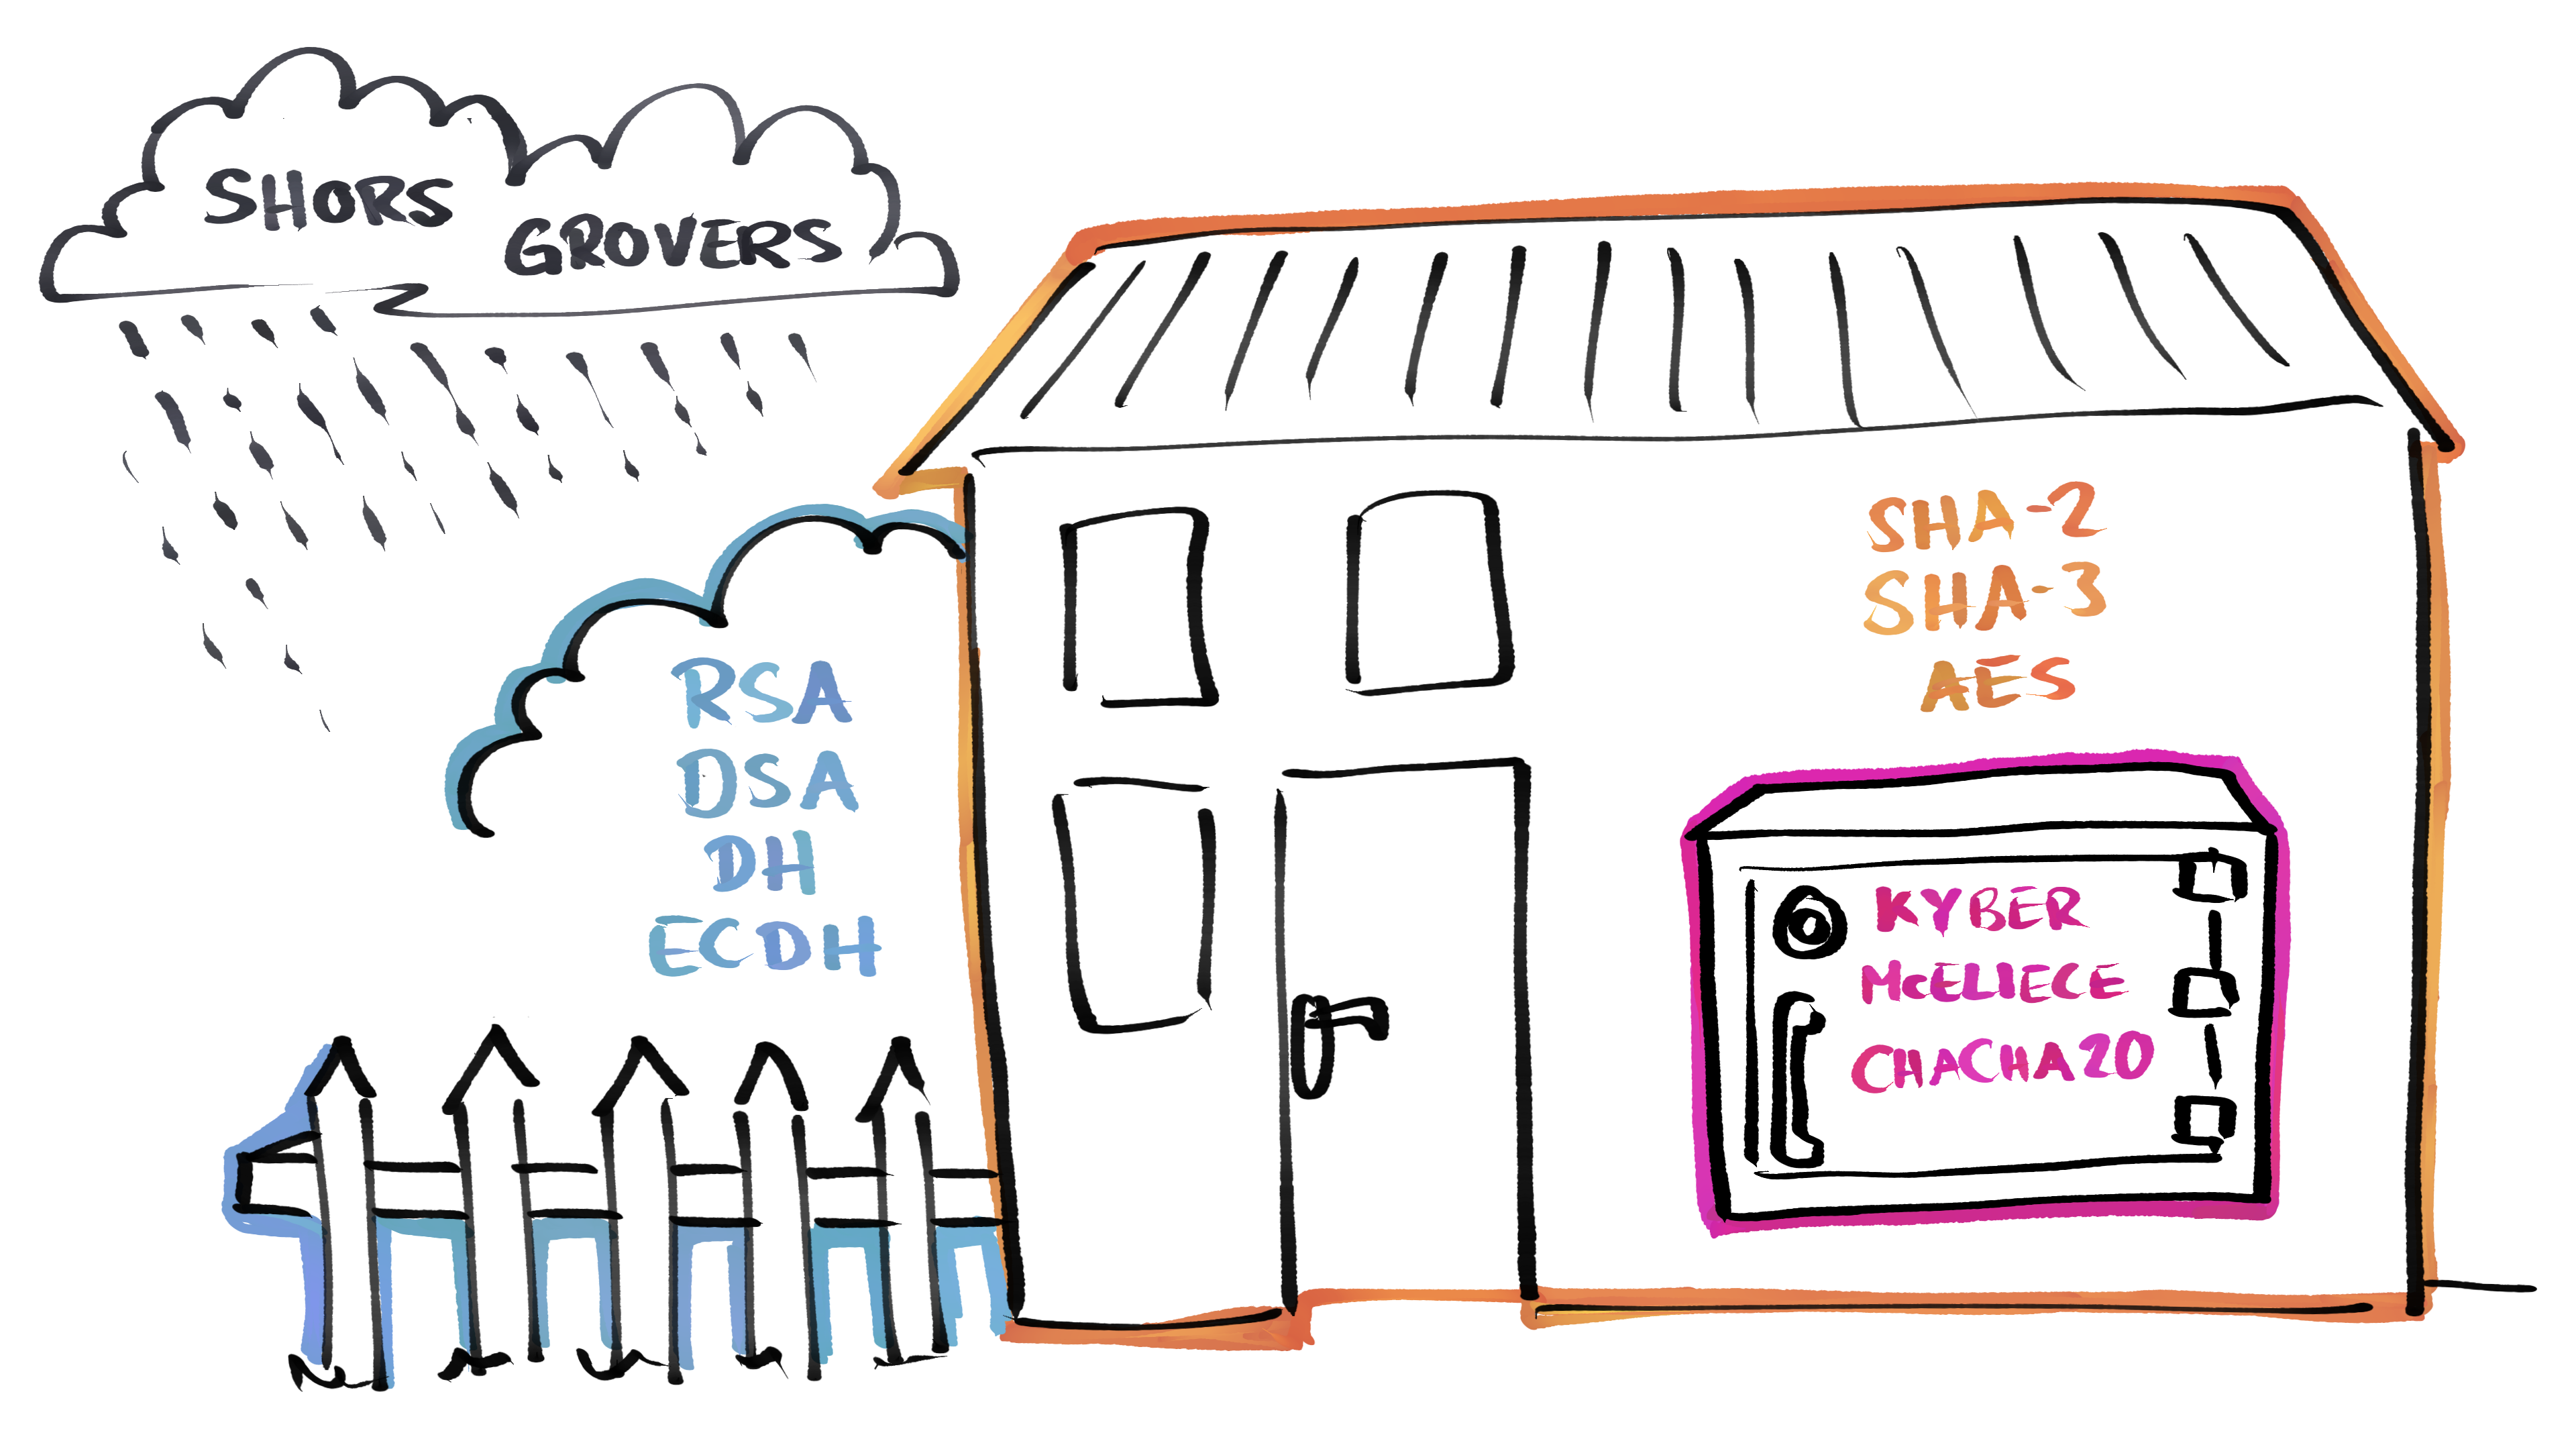
\includegraphics[width=1.5\linewidth]{graphics/qc and crypto.png}
}%
\par
\imgNote{\makebox[\linewidth][r]{Quantencomputer überschatten Kryptografieverfahren.}}
\end{column}
\end{columns}
\end{frame}
		
\begin{frame}{PQ-sichere VPNs: WireGuard + Rosenpass}
  \begin{itemize}
    \item  Hybride Sicherheit

    \begin{itemize}
      \item Bricht nur, wenn Rosenpass \textbf{und} WireGuard versagen
    \end{itemize}
    \item  Überall nutzbar, wo WireGuard schon läuft
    \item  Ohne Anpassung vom WireGuard Source Code

    \begin{itemize}
      \item Shared Secret aus Rosenpass = PSK für WireGuard
    \end{itemize}
    \item  Aber:

    \begin{itemize}
      \item Ein Prozess mehr
      \item Handshake alle 2 Minuten
    \end{itemize}
  \end{itemize}

\makebox[\linewidth][c]{%

\includegraphics[width=.6\linewidth]{graphics/wireguard and rp.png}}

\imgNote{\makebox[\linewidth][c]{WireGuard mit Rosenpass.}}
\end{frame}

\begin{frame}{Rosenpass: Sicherheitseigenschaften}

\vspace{0.5em}
\begin{columns}[t]
\begin{column}{.30\textwidth}
\heading{WireGuard}
\begin{itemize}
  \itemtick Session-key secrecy
  \itemtick \dots
  \itemtick Identity Hiding
  \itemfail \textbf{Non-Interruptability} \footnote[frame]{Angenommen der Systemzeit wird Vertraut}
  \itemfail \textbf{Post-Quantum Security}
\end{itemize}
\end{column}

\begin{column}{.30\textwidth}
\heading{
  PQ WireGuard
  \footnote[frame]{
	  Hülsing, Ning, Schwabe, Weber, Zimmermann. “Post-quantum WireGuard”. https://ia.cr/2020/379
	}
}
\begin{itemize}
  \itemtick \textbf{Post-Quantum Security}
  \itemfail \textbf{Hybrid security}
  \itemfail \textbf{Non-Interruptability} \footnote[frame]{Assuming a PSK}
\end{itemize}
\end{column}

\begin{column}{.30\textwidth}
\heading{Rosenpass}
\begin{itemize}
  \itemtick \textbf{Non-Interruptability} \footnote[frame]{Through cookies}
  \itemtick \textbf{Hybrid security} \footnote[frame]{Wenn es mit WireGuard benutzt wird}
\end{itemize}
\end{column}

\end{columns}
\vspace{1.5em}

\end{frame}

\begin{frame}{Zum Nachbauen… aus dem Whitepaper:}
  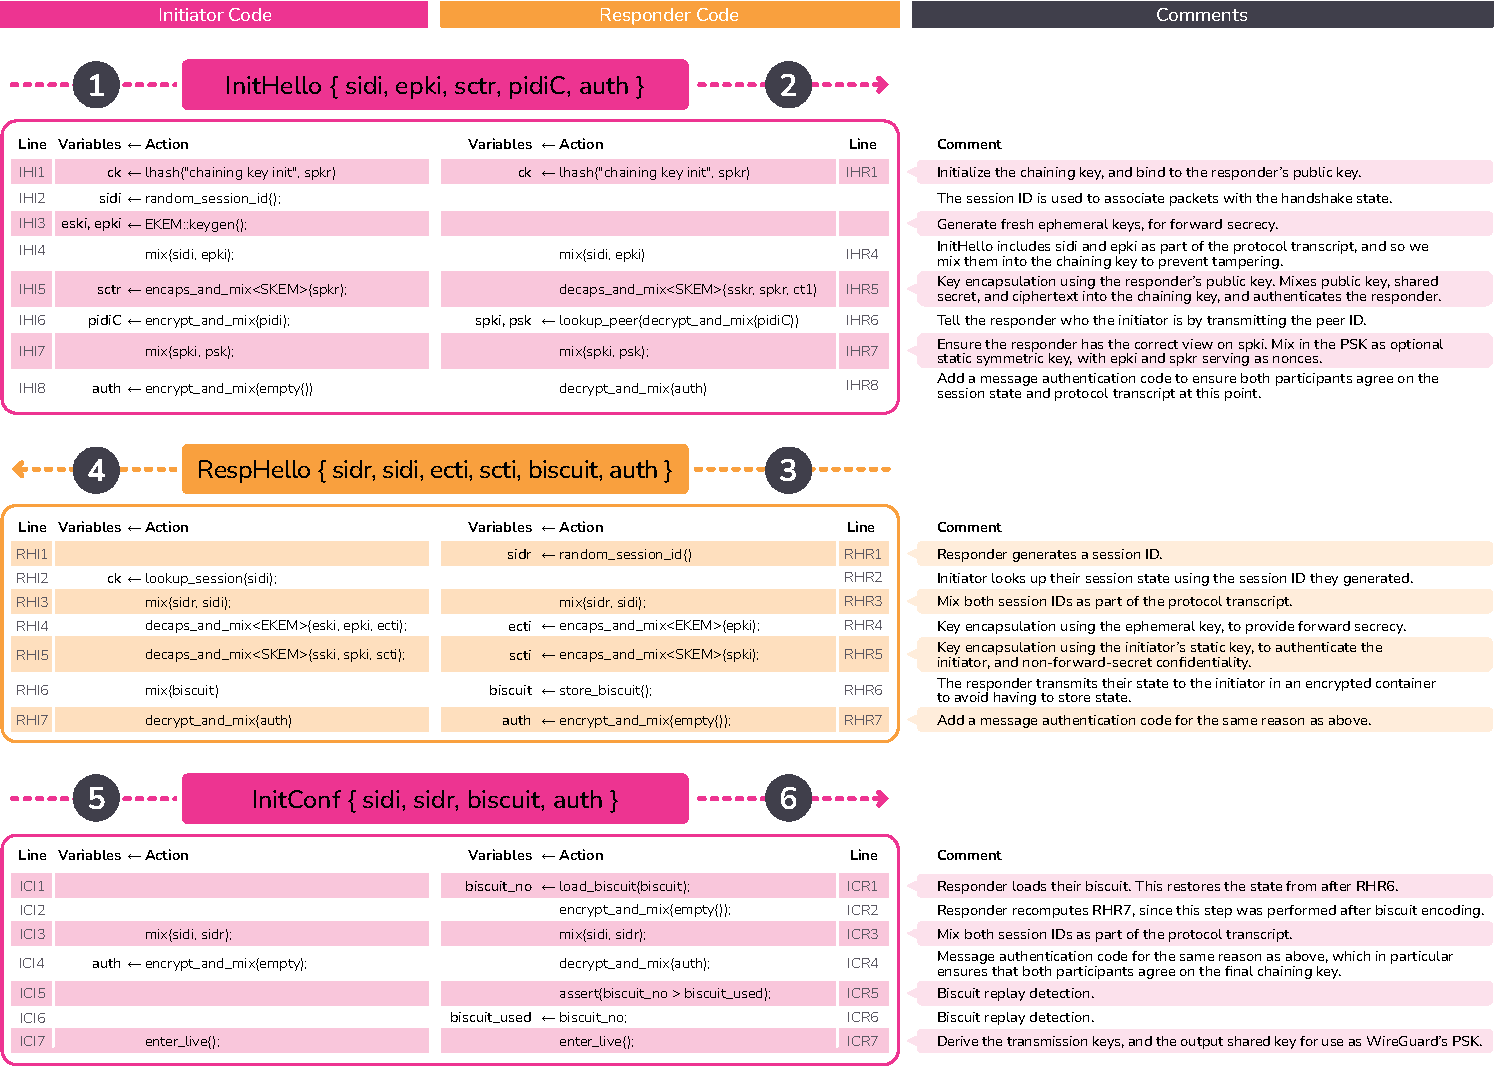
\includegraphics[height=.9\textheight]{graphics/rosenpass-wp-message-handling-code.pdf}
\end{frame}

\begin{frame}{Zum Nachbauen… go-rosenpass – Steffen Vogel FTW}
  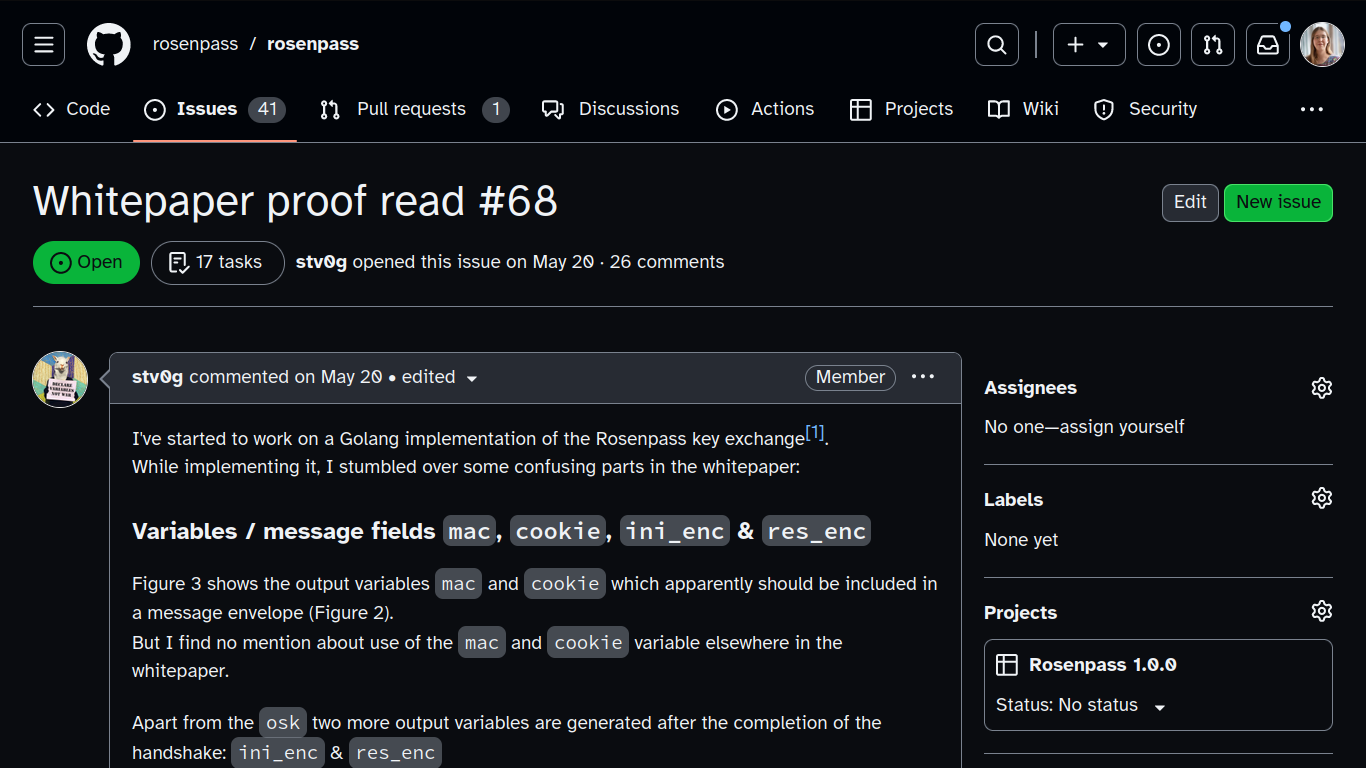
\includegraphics[height=.9\textheight]{assets/2023-09-02-steffen-proof-read.png}
\end{frame}

\begin{frame}{Zum Nachbauen… go-rosenpass – Steffen Vogel FTW}
  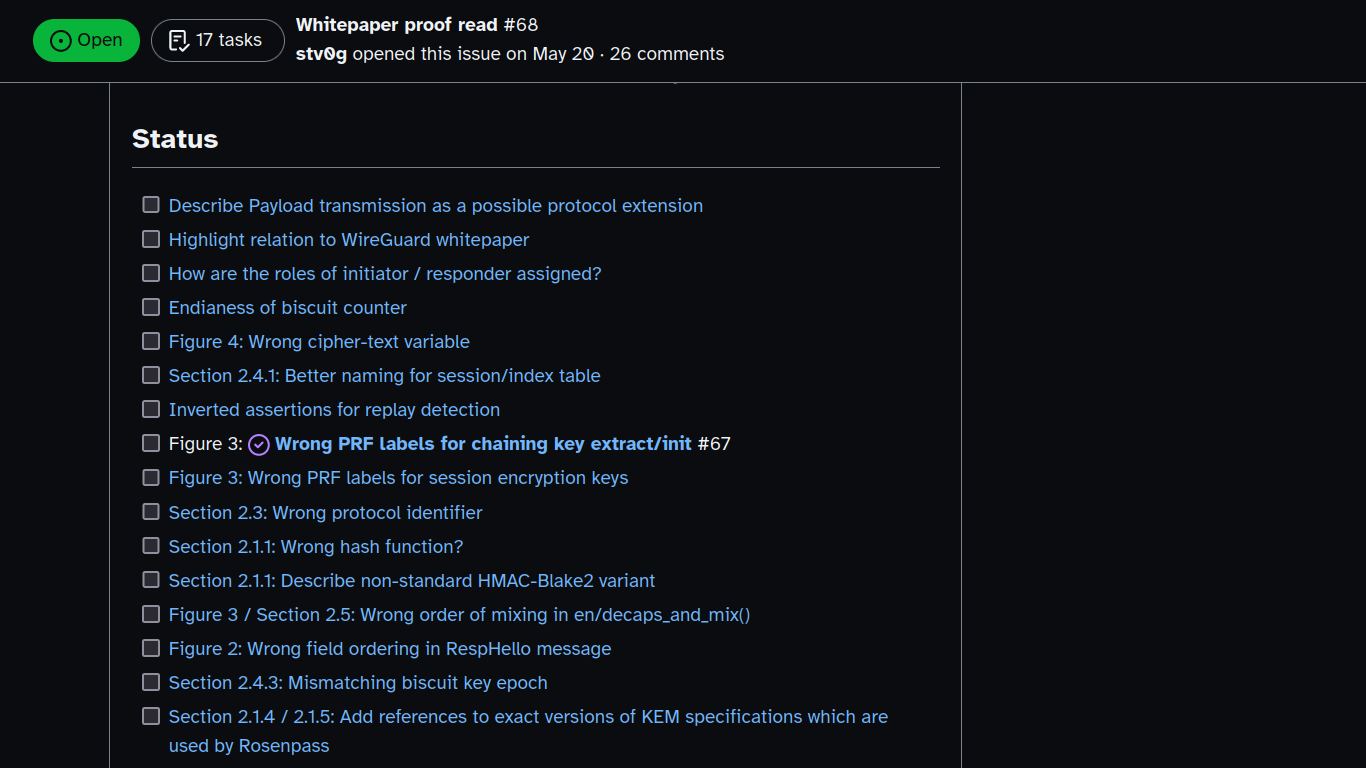
\includegraphics[height=.9\textheight]{assets/2023-09-02-steffen-proof-read-issues.png}
\end{frame}

\begin{frame}{Zum Integrieren… NetBird}
  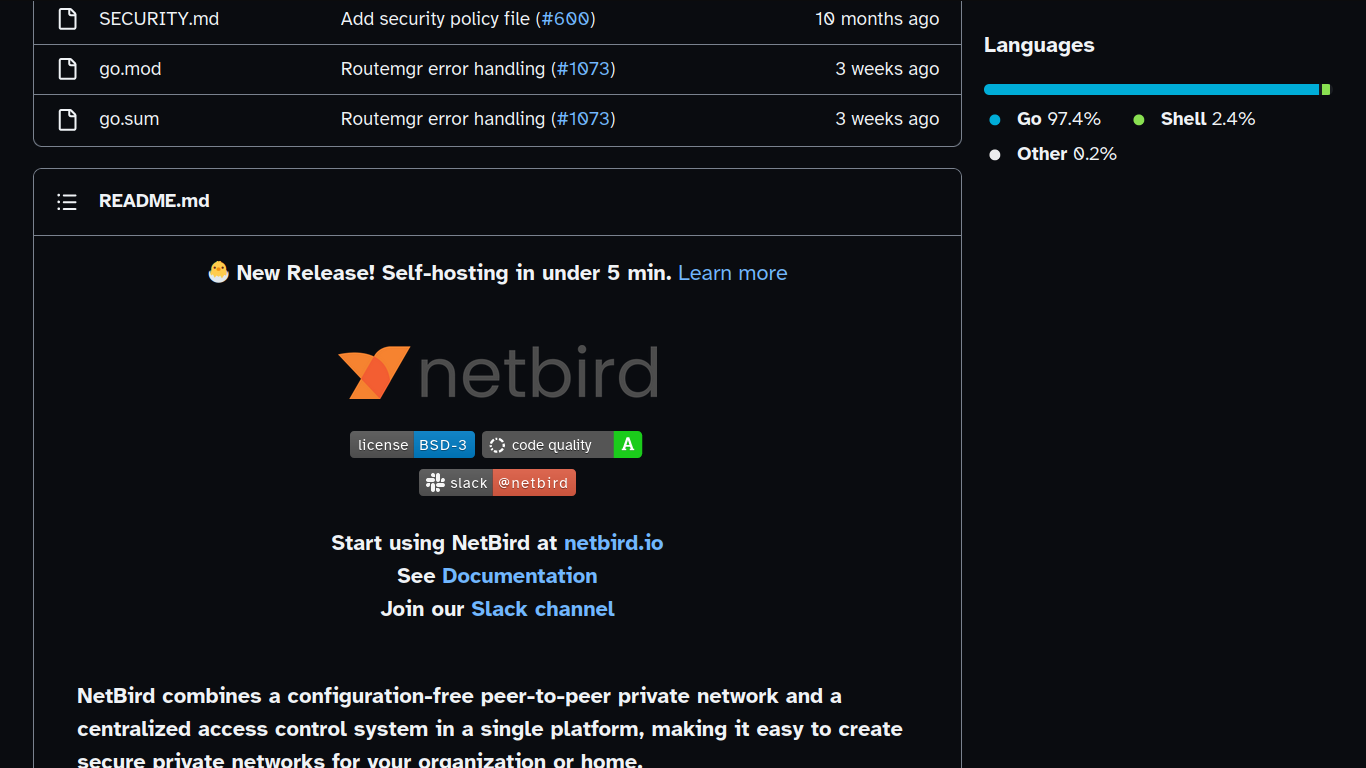
\includegraphics[height=.9\textheight]{assets/2023-09-02-netbird-gh.png}
\end{frame}

\begin{frame}{Zum Integrieren… NetBird}
  
\includegraphics[height=.9\textheight]{assets/2023-09-02-netbird-gh-rosenpass-testemonial.png}
\end{frame}

\begin{frame}{Zum Integrieren… NetBird}
\begin{columns}[c]
\begin{column}{0.7\textwidth}
  \begin{itemize}
    \item Netbird: Einfaches user interface
    \item Rosenpass: Hochsichere PQ-Crypto
    \item
      go-rosenpass: Um Plattformen zu unterstützen auf denen die Rust Variante schwer zu integrieren ist
      \begin{itemize}
        \item Android
        \item iOS
        \item Windows
        \item \dots
      \end{itemize}
  \end{itemize}
\end{column}

\begin{column}{0.2\textwidth}
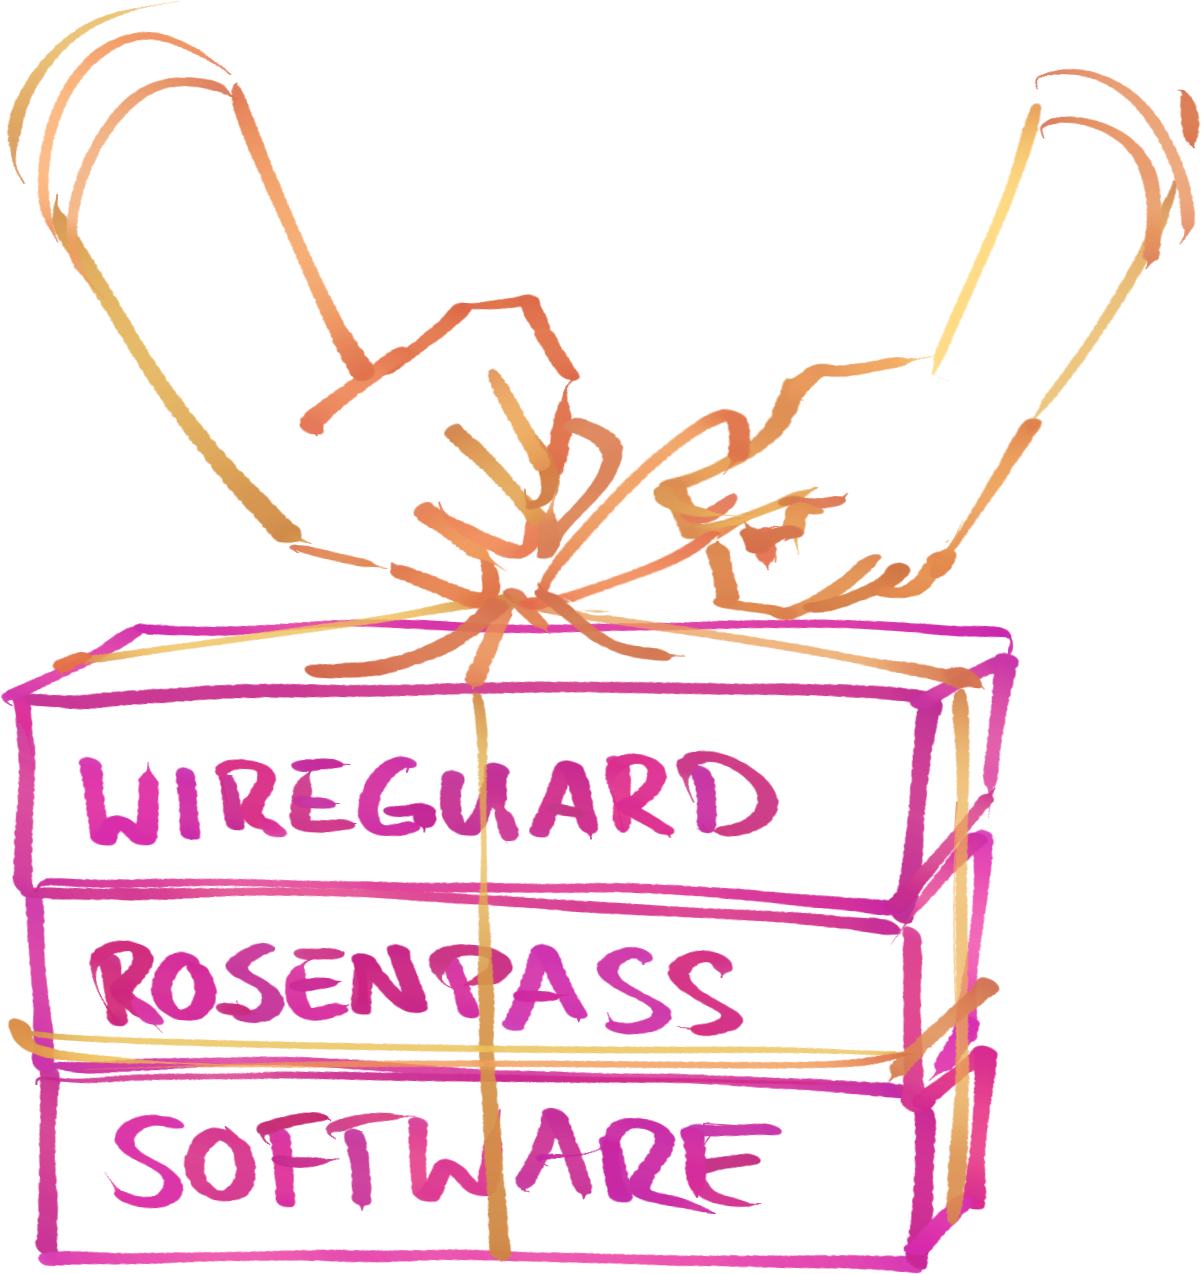
\includegraphics[width=\linewidth]{graphics/rosenpass in anderen apps.png}

\medskip
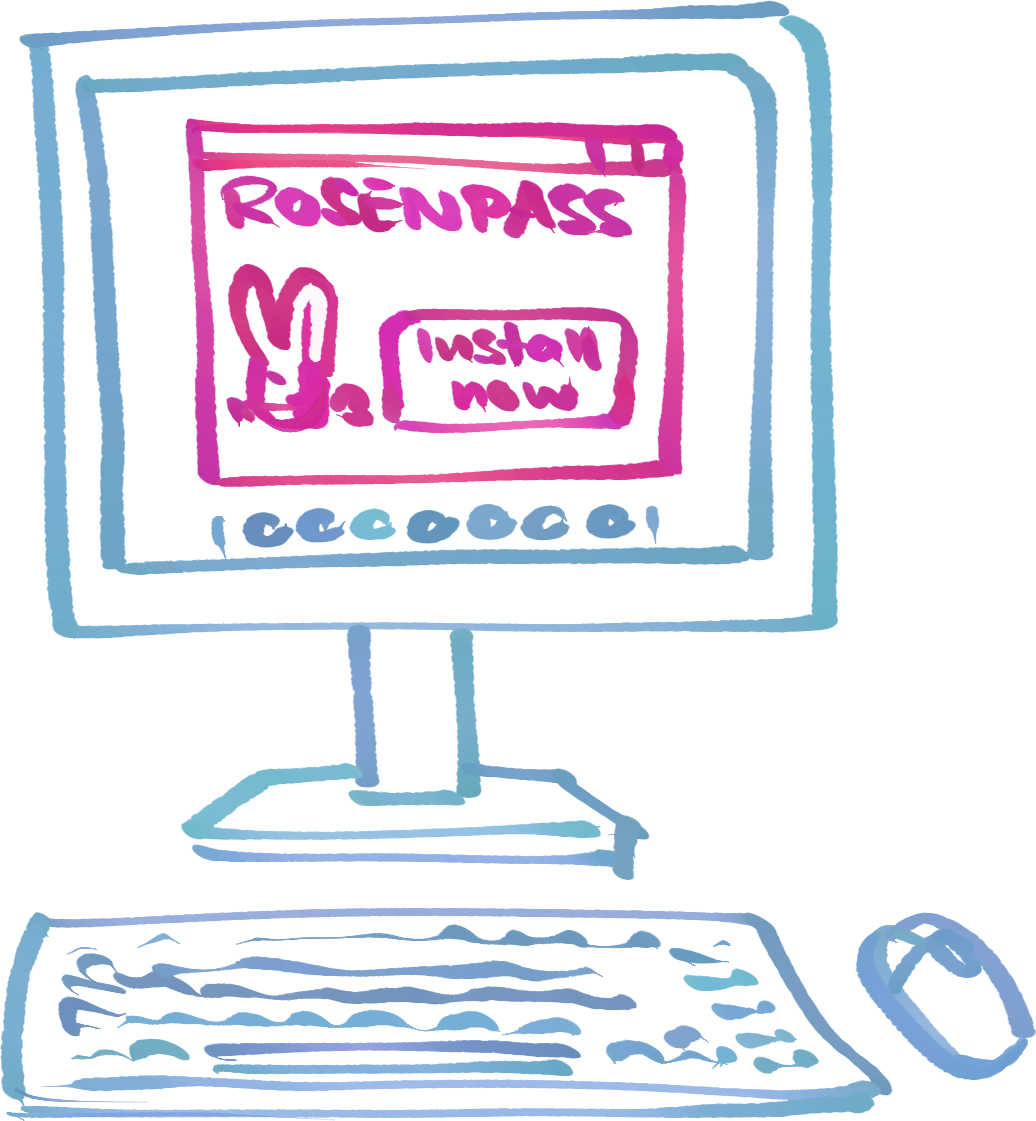
\includegraphics[width=\linewidth]{graphics/Illu-install.png}

\end{column}
\end{columns}
\end{frame}

\begin{frame}{Zum Integrieren… Prototypefund 14 Projekt}
\begin{columns}[c]
\begin{column}{0.7\textwidth}
  \begin{itemize}
    \item Schnittstelle zwischen Komponenten
    \item Kommunikation über Unix-Sockets
    \item Spezielle Serialisierungsbibliothek für Schlüsseldaten\footnotemark
    \item Broker-Pattern für Rosenpass– Jede Komponente in einem eigenen Prozess
    \item Mikro-VMs um wirklich hohe sicherheit zu haben
    \item Minimale Privilegien; Sandboxing
  \end{itemize}
\end{column}

\begin{column}{0.2\textwidth}
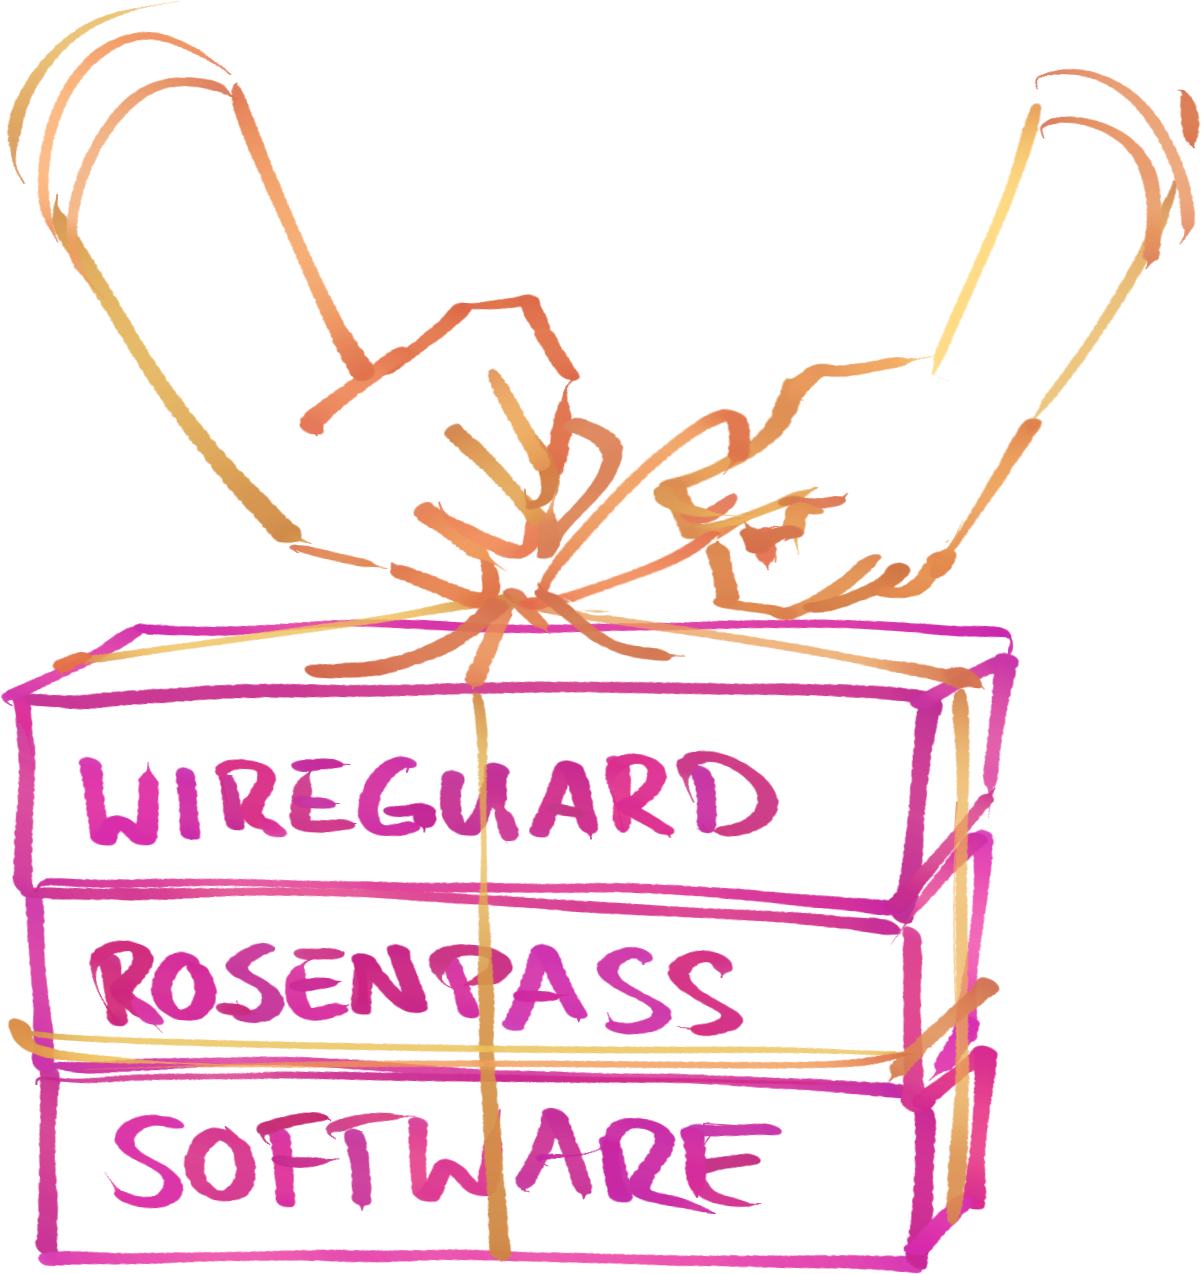
\includegraphics[width=\linewidth]{graphics/rosenpass in anderen apps.png}

\medskip
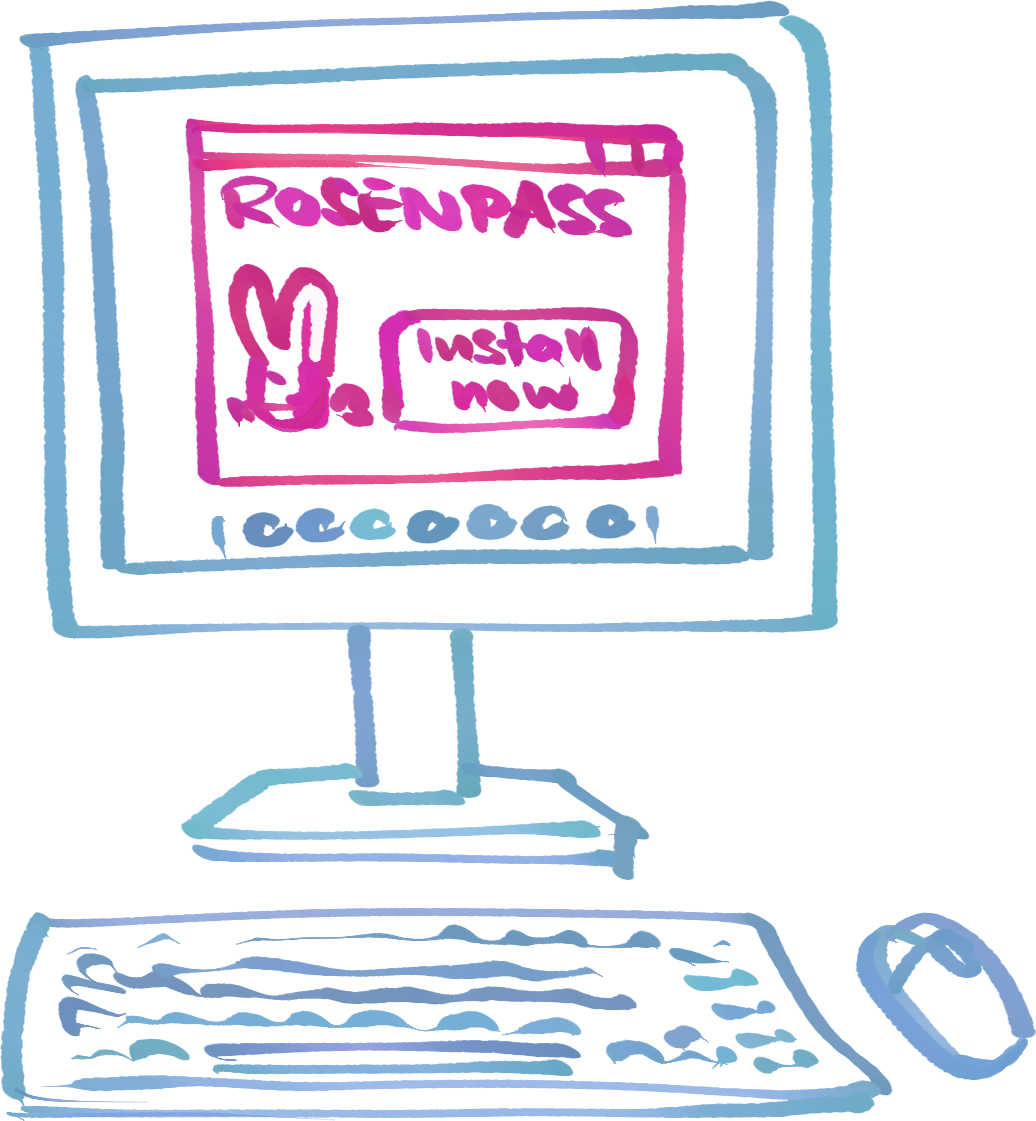
\includegraphics[width=\linewidth]{graphics/Illu-install.png}

\end{column}
\end{columns}

\footnotetext{Externes Memory-Management}

\end{frame}

\begin{frame}{Rosenpass Roadmap}
\begin{columns}[c]
\begin{column}{0.7\textwidth}
\begin{itemize}
  \item Sicherheitsbeweis
  \item Formelle Verifikation der Implementierung
  \item Separakte Komponenten? Zertifikate, Schlüsseltausch und verschlüsselte Verbindung
  \item Vereinfachung

  \item  Kryptografie + Safety Forschung:
  \begin{itemize}
    \item Kryptografie in der Avionik
    \item Decryption Despite Error
  \end{itemize}
\end{itemize}
\end{column}

\begin{column}{0.2\textwidth}
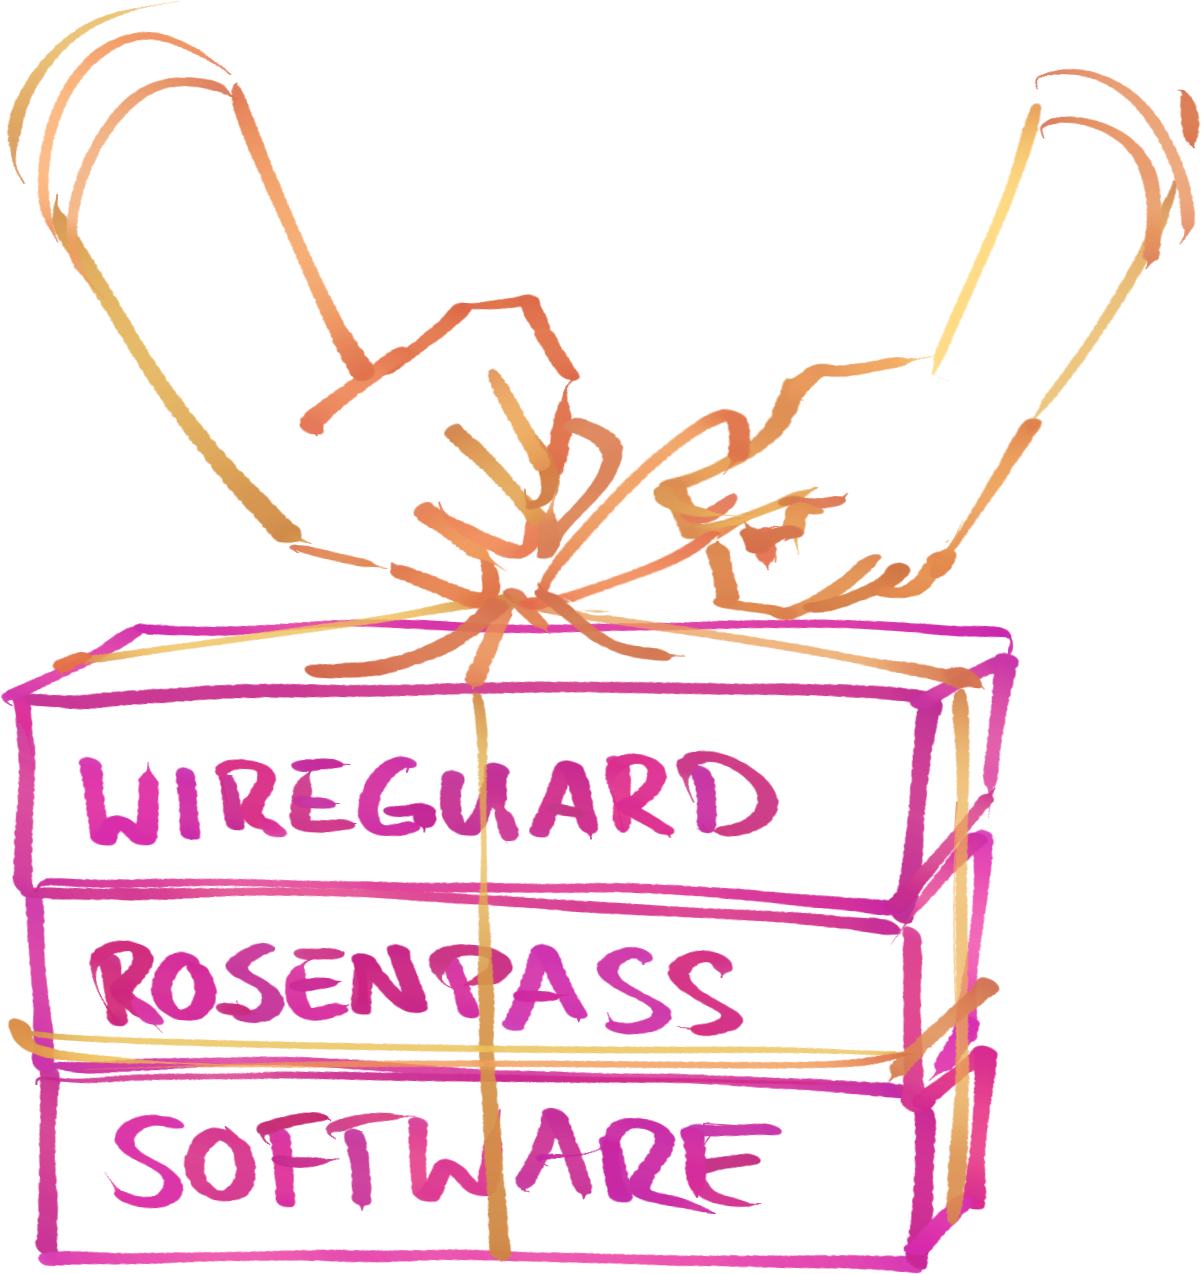
\includegraphics[width=\linewidth]{graphics/rosenpass in anderen apps.png}

\medskip
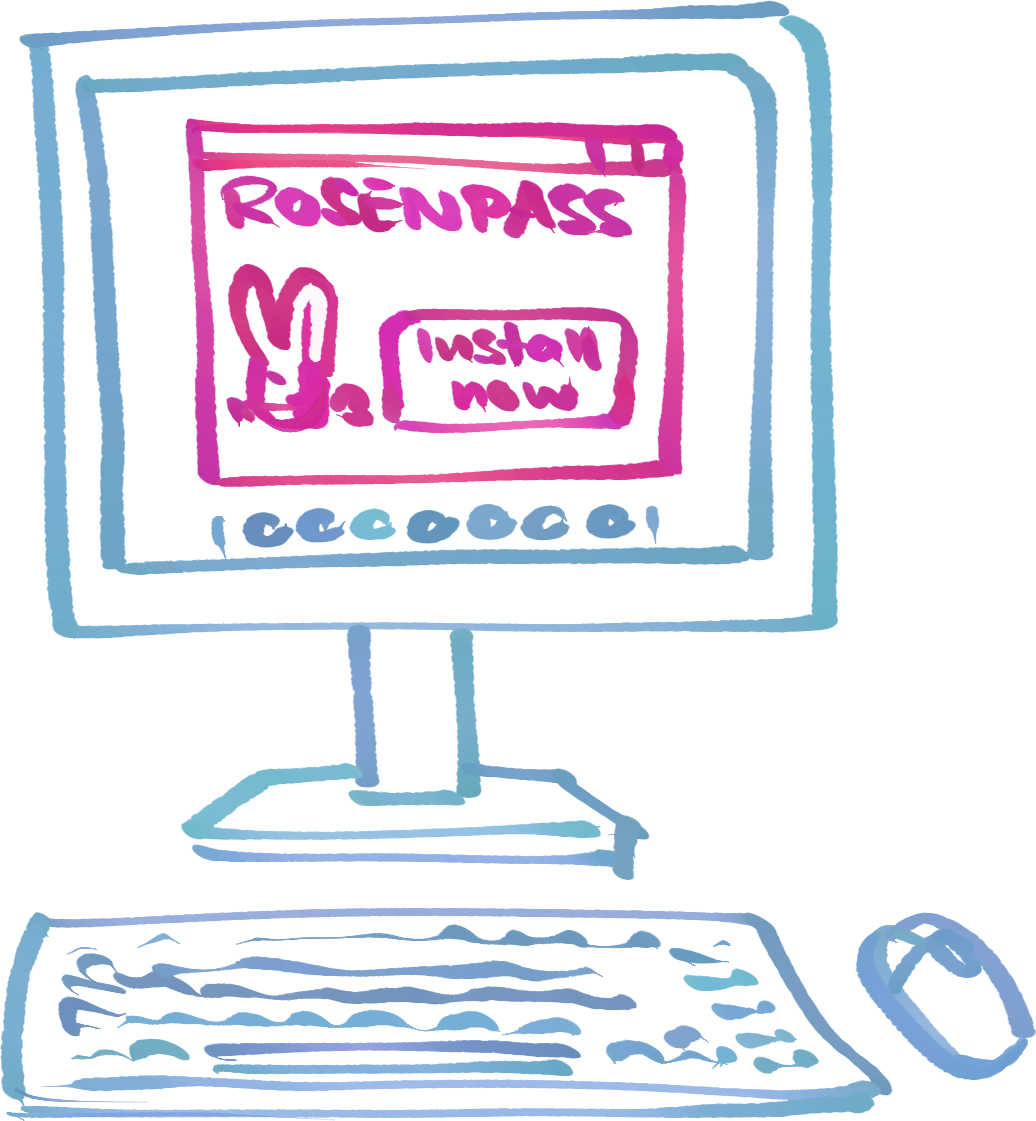
\includegraphics[width=\linewidth]{graphics/Illu-install.png}

\end{column}
\end{columns}
\end{frame}

\begin{frame}{Rosenpass Struktur}
\begin{columns}[c]
\begin{column}{0.7\textwidth}
\begin{itemize}
  \item Zusammenkunft von Kryptografie, Dev und SciComm Experten
  \item Zusammenarbeit mit Industrie
  \item Ansprechpartner für Integratoren
  \item Antihirarchisches Arbeiten
  \item Mit mehreren Firmen arbeiten; Open-Source R\&D
  \item Translationsforschung: Schnittstelle zwischen Industrie und Wissenschaft
  \item Karo hätte gerne mal wieder Freizeit
\end{itemize}
\end{column}

\begin{column}{0.2\textwidth}
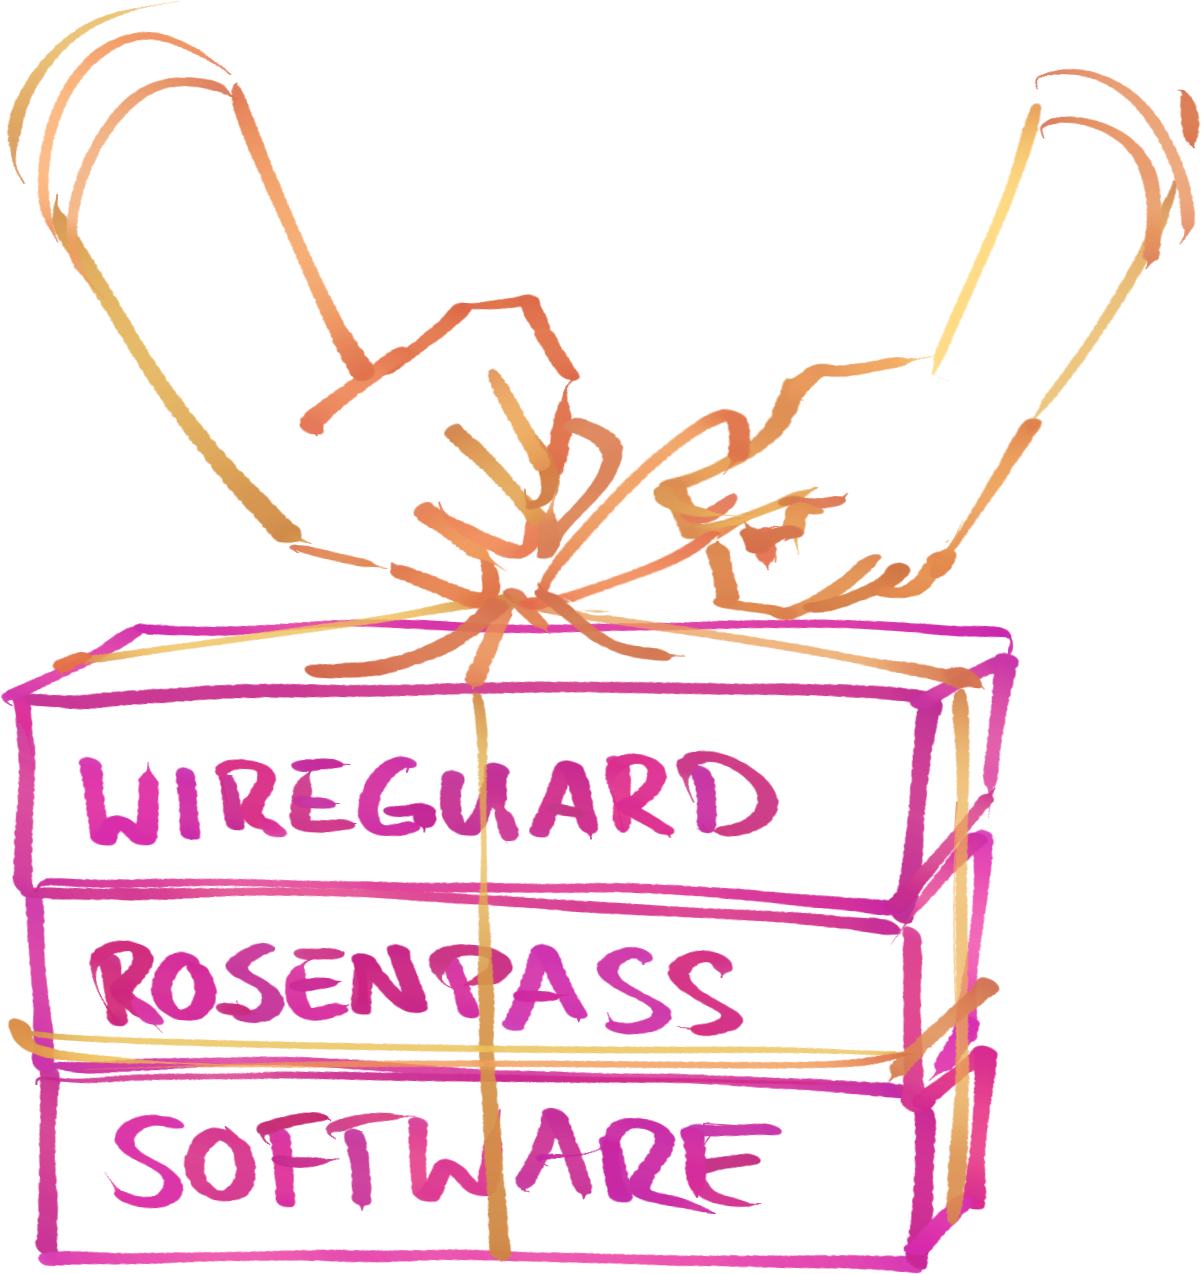
\includegraphics[width=\linewidth]{graphics/rosenpass in anderen apps.png}

\medskip
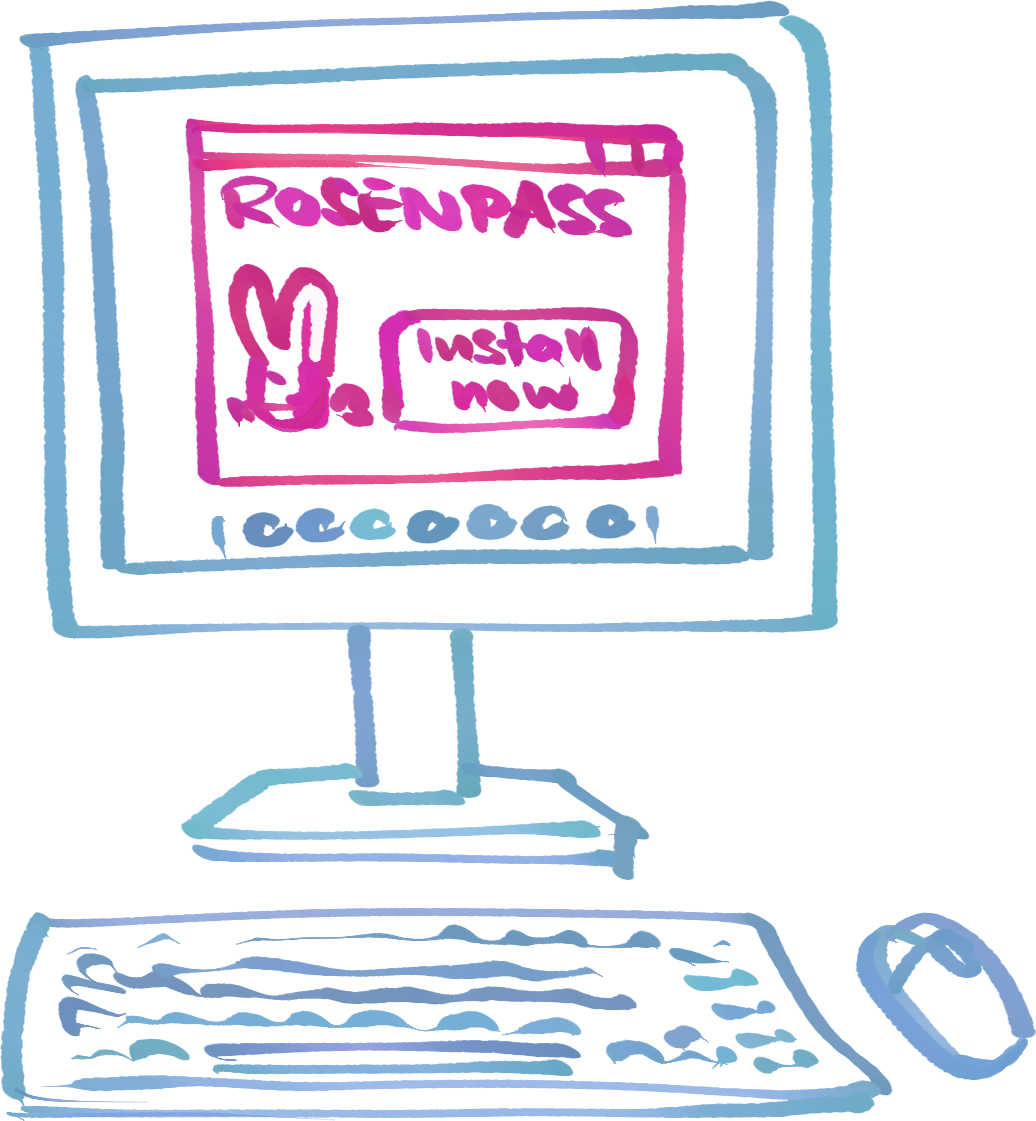
\includegraphics[width=\linewidth]{graphics/Illu-install.png}

\end{column}
\end{columns}
\end{frame}

\begin{frame}{Idee: Kryptografie als Notar Erklären}
\begin{columns}[c]

\begin{column}{0.7\textwidth}
  \begin{itemize}
    \item Problem: Kryptografie wird als schwarze Magie verstanden
    \item Problem: Krude vorschläge zur Verwaltungsautomatisierung
    \item Problem: Und Strafverfolgung
    \item Problem: Krypto wird auf Verschlüsselung reduziert
    \item
      Problem: Kaum jemand weiß was moderne Verfahren tun
      \begin{itemize}
        \item Elliptic-Curve Pairings
        \item Multi-Party Computation
        \item Homomorphische Verschlüsselung
        \item Dankenbanken mit anonymem Zugriff
        \item Anonyme Kommunikation
      \end{itemize}
  \end{itemize}
\end{column}

\begin{column}{0.2\textwidth}
  \ImgSource{
    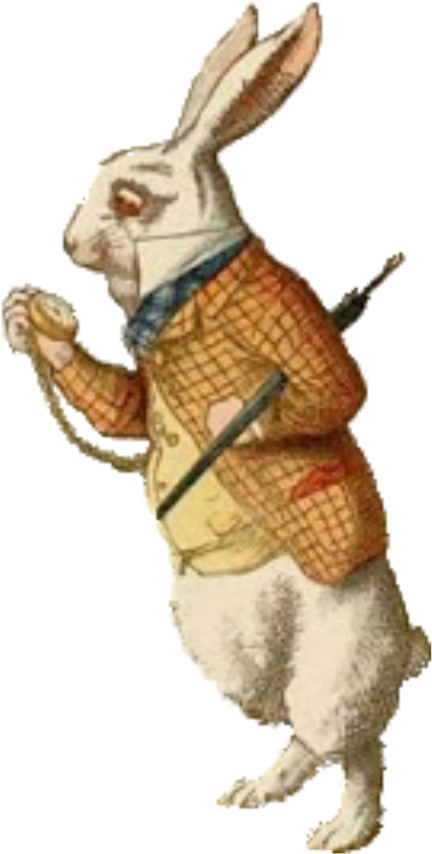
\includegraphics[height=.5\textheight]{assets/rabbit-with-clock.png}
  }{White Rabbit aus Alice in Wonderland – CC0}
  \imgNote{Häßchen sind die besseren Menschen.}
\end{column}

\end{columns}
\end{frame}

\begin{frame}{Idee: Kryptografie als Notar Erklären}
\begin{columns}[c]

\begin{column}{0.7\textwidth}
  \begin{itemize}
    \item Krypto: Einsatzfähig für viele Prozesse in denen Information Übertragen wird
    \item Datenschutz: Anonyme, Nutzergesteuerte Prozesse
    \item Idee: Metapher von Kryptografie als Notar
      \begin{itemize}
        \item Notare werden Bestraft wenn sie Dinge Zusichern die sie nicht können
        \item Oder wenn sie gegen Regeln verstoßen
        \item Spezieller schutz vor dem Recht
        \item Kryptografie: Ähnlich, nur Matematisch, statt mit Staatsgewalt
      \end{itemize}
  \end{itemize}
\end{column}

\begin{column}{0.2\textwidth}
  \ImgSource{
    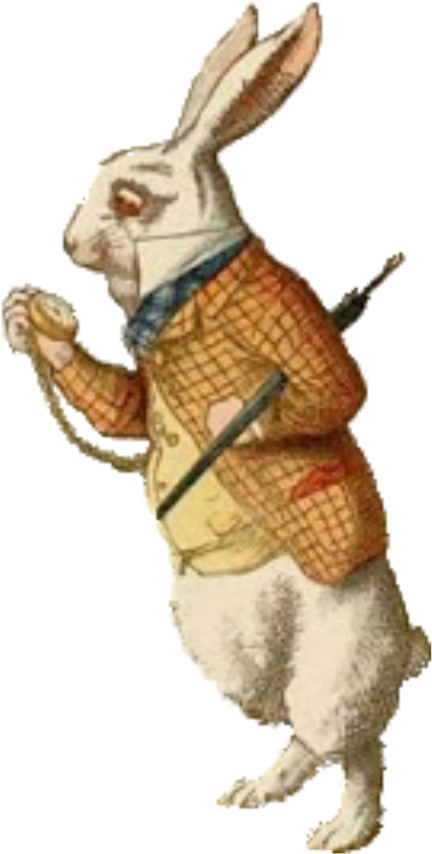
\includegraphics[height=.5\textheight]{assets/rabbit-with-clock.png}
  }{White Rabbit aus Alice in Wonderland – CC0}
  \imgNote{Häßchen sind die besseren Menschen.}
\end{column}

\end{columns}
\end{frame}

\end{document}
